\documentclass[tikz,border=10pt]{standalone}
\usetikzlibrary{positioning,arrows.meta}
\definecolor{eventFill}{HTML}{FFE0B2}
\definecolor{eventBorder}{HTML}{FB8C00}
\definecolor{subjectFill}{HTML}{C8E6C9}
\definecolor{subjectBorder}{HTML}{4CAF50}
\definecolor{observerFill}{HTML}{E1BEE7}
\definecolor{observerBorder}{HTML}{9C27B0}

\begin{document}
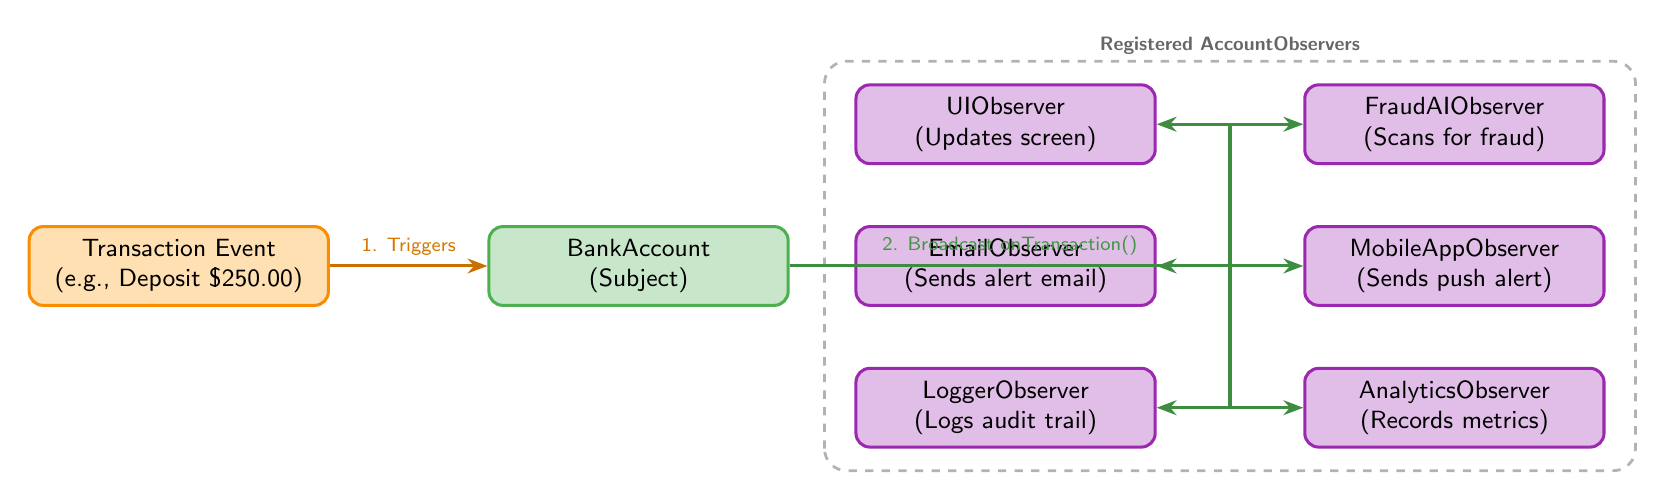
\begin{tikzpicture}[
    block/.style={
        rectangle, draw,
        minimum width=3.8cm, minimum height=1.0cm,
        align=center,
        text centered, rounded corners=5pt,
        line width=1.1pt, font=\sffamily\small
    },
    arrow/.style={-{Stealth[scale=0.9]}, line width=1.1pt}
]
  % Left Side nodes
  \node[block, fill=eventFill, draw=eventBorder] (event) {Transaction Event\\(e.g., Deposit \$250.00)};
  
  \node[block, fill=subjectFill, draw=subjectBorder, right=2.0cm of event] (subject) {BankAccount\\(Subject)};
  
  % Symmetrical Observer Columns: Column 1 (Left), Column 2 (Right)
  % We place Column 1 left of center, Column 2 right of center, centering around x=13.35.
  \node[block, fill=observerFill, draw=observerBorder] (obs_ui) at (10.5, 1.8) {UIObserver\\(Updates screen)};
  \node[block, fill=observerFill, draw=observerBorder] (obs_email) at (10.5, 0) {EmailObserver\\(Sends alert email)};
  \node[block, fill=observerFill, draw=observerBorder] (obs_log) at (10.5, -1.8) {LoggerObserver\\(Logs audit trail)};
  
  \node[block, fill=observerFill, draw=observerBorder] (obs_fraud) at (16.2, 1.8) {FraudAIObserver\\(Scans for fraud)};
  \node[block, fill=observerFill, draw=observerBorder] (obs_mobile) at (16.2, 0) {MobileAppObserver\\(Sends push alert)};
  \node[block, fill=observerFill, draw=observerBorder] (obs_analytics) at (16.2, -1.8) {AnalyticsObserver\\(Records metrics)};

  % Boundary Box for Observers
  \draw[dashed, draw=gray!60, line width=1pt, rounded corners=8pt] 
      (8.2, -2.6) rectangle (18.5, 2.6);
  \node[font=\sffamily\bfseries\scriptsize, text=gray!80!black] at (13.35, 2.8) {Registered AccountObservers};

  % Event to BankAccount arrow
  \draw[arrow, draw=eventBorder!80!black] (event) -- (subject) 
      node[midway, above, font=\sffamily\scriptsize, text=eventBorder!85!black] {1. Triggers};
  
  % BankAccount to Central Bus
  % Central distribution bus is at x = 13.35
  \draw[line width=1.1pt, draw=subjectBorder!80!black] (subject.east) -- (13.35, 0)
      node[midway, above, font=\sffamily\scriptsize, text=subjectBorder!85!black] {2. Broadcast onTransaction()};
      
  % Vertical distribution bus line
  \draw[line width=1.1pt, draw=subjectBorder!80!black] (13.35, 1.8) -- (13.35, -1.8);
  
  % Distribution arrows pointing outwards to observers
  % Left Column (connects to east side of nodes)
  \draw[arrow, draw=subjectBorder!80!black] (13.35, 1.8) -- (obs_ui.east);
  \draw[arrow, draw=subjectBorder!80!black] (13.35, 0) -- (obs_email.east);
  \draw[arrow, draw=subjectBorder!80!black] (13.35, -1.8) -- (obs_log.east);
  
  % Right Column (connects to west side of nodes)
  \draw[arrow, draw=subjectBorder!80!black] (13.35, 1.8) -- (obs_fraud.west);
  \draw[arrow, draw=subjectBorder!80!black] (13.35, 0) -- (obs_mobile.west);
  \draw[arrow, draw=subjectBorder!80!black] (13.35, -1.8) -- (obs_analytics.west);

\end{tikzpicture}
\end{document}